\section{Método factoría}

\begin{figure}[ht!]
\begin{center}
	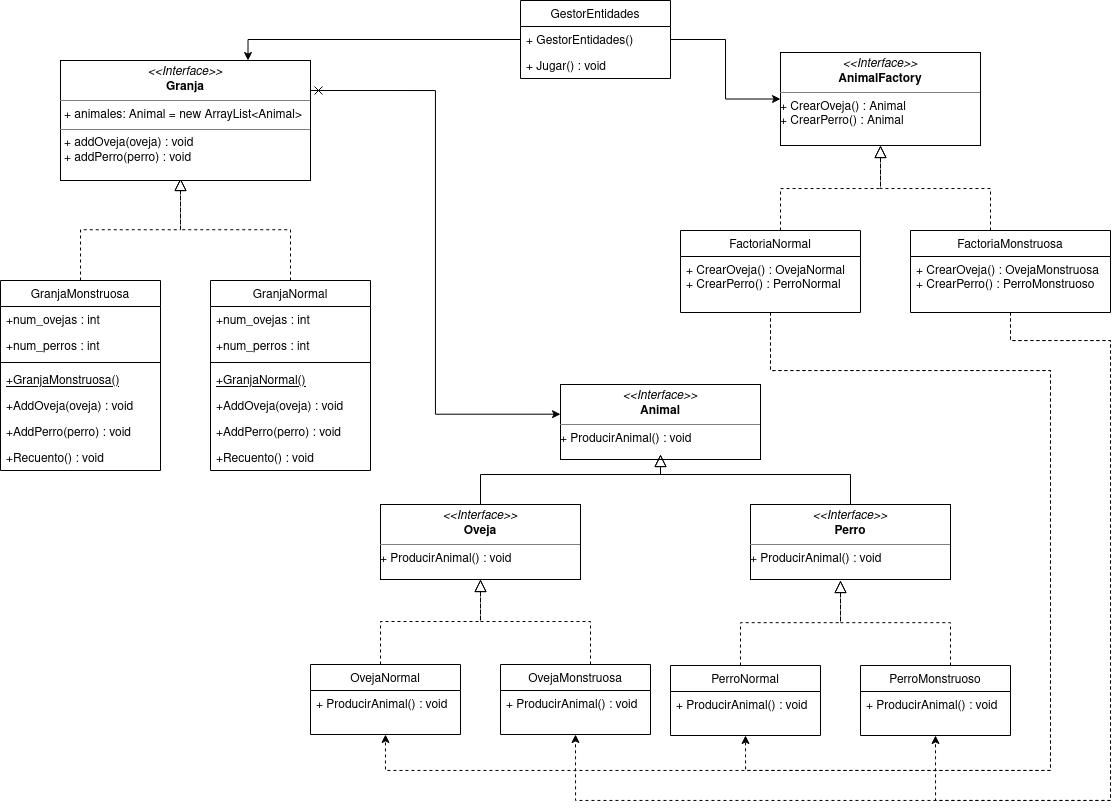
\includegraphics[scale=0.35]{DiagramaFactoria}
\end{center}
\caption{Diagrama UML de la aplicación del patrón \textit{Método Factoría}.}
\end{figure}

Hemos aplicado el patrón de diseño \textit{Método Factoría} sobre el sistema de gestión de entidades de \textit{CaveArt}, particularmente para la creación de granjas de animales.

Este procedimiento sería también aplicable a la generación de otras entidades pacíficas y hostiles, pero nos hemos decantado por este caso particular dado el valor añadido del concepto de la Granja. Además, estos otros casos serían más \textit{straightforward} y, por tanto, triviales.

El programa consiste en dos hebras concurrentes que llenan dos granjas: una \texttt{GranjaNormal}, habitada por ovejas y perros normales; y una \texttt{GranjaMonstruosa}, habitada por ovejas y perros monstruosos, hostiles al jugador.

Cada hebra del \texttt{GestorEntidades} llama a una factoría: \texttt{FactoriaNormal} o \texttt{FactoriaMonstruosa}. Estas factorías son implementaciones de la interfaz \texttt{AnimalFactory}. Se escoge de forma aleatoria si se generará una oveja o un perro, y la factoría llama al método \texttt{crearOveja} o \texttt{crearPerro} . Estos métodos, a su vez, llamarán al constructor del animal escogido.
